% !TeX spellcheck = en_US

\chapter{Analysis}
The Analysis shows use-cases for the system based on the stakeholders. A gap-analysis is performed to compare use-cases of the new system in difference to the old one. The result of this process will be requirements, which are separated into functional and non-functional.


\section{Stakeholders}
Stakeholders are groups of people that have an interest in the system. This can be from a practical, or from a business standpoint.

\subsection{Model Developer}
The Model Developer is a technical user that creates a MARS model in cooperation with a domain expert. His main goal, is to make sure the model executes correctly and without errors.

\subsection{Simulation Creator}
The Model Developer is an domain export. He Uses the Model, created by the Model Developer to answer a research question. Model Developers goal is, to start various simulations with a given model to validate or invalidate theories.

\subsection{Group Administrator}
The Group Admin is a user of the system with a leading roll in his group. He wants to manage people belonging to a particular group and handle group dependent settings. He wants to add users to his group, remove them and handle permissions for data, owned by his group.

\subsection{Administrator}
The Administrator is a global acting user with far reaching permission inside the system. An admin has to be able to alter any kind of data inside the system. Due to his wide range of capabilities, he has to be a trusted to act responsibly with the given responsibilities.


\section{Use-cases}
The workflow that includes completing all the necessary steps to start a simulation can be broken down into five parts: \textit{Import Data}, \textit{Check imported Files}, \textit{Create Mapping}, \textit{Start Simulation} and \textit{View Results}.\\
The additional Use-cases \textit{Manage Groups} and \textit{Manage Users} are for administrative purposes only. Figure \ref{fig:use-cases} shows an overview of the Use-cases with their stakeholders.\\
This piece of work does not cover the whole workflow. Instead, it is focused on the highlighted area of the image. In the following chapters, only these parts will be covered.\\
Although the Model Developer and the Simulation Creator have a different view of the Websuite, the Use-Cases do not differ. This is why they are simply referred as User.
\begin{figure}[H]
	\centering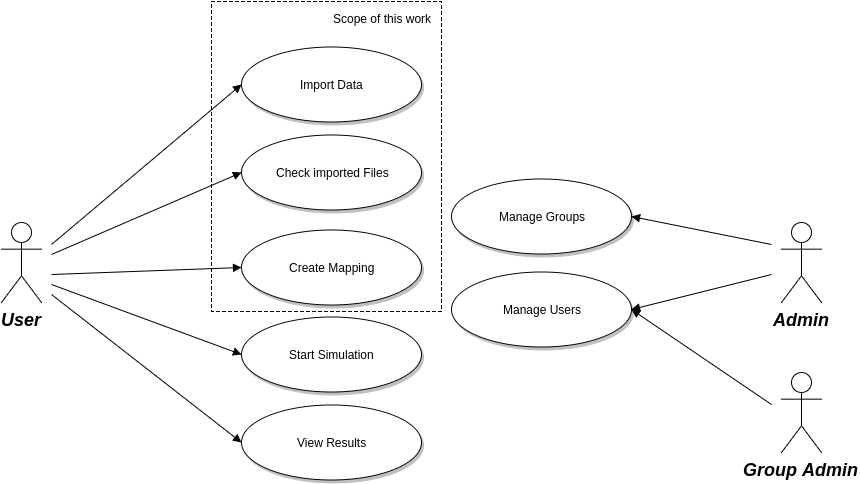
\includegraphics[width=1\textwidth]{res/Use-Cases_reduced}
	\caption{Use-Cases in UML notation}
	\label{fig:use-cases}
\end{figure}

\subsection{Import}
\begin{usecase}
	\addtitle{Import I}{Data}
	\addfield{Summary}{Upload local data files to the Websuite, to use them for a simulation.}
	\additemizedfield{Actors}{
		\item User
	}
	\additemizedfield{Preconditions}{
		\item Import data page is open.
	}
	\additemizedfield{Primary Scenario: }{
		\item The user drags one or multiple files onto the upload window, fills the form for every file and starts the import.
	}
	\additemizedfield{Alternative Scenario: }{
		\item The user clicks the upload button, fills the form for every file and starts the import.
	}
\end{usecase}

\begin{usecase}
	\addtitle{Import II}{Model}
	\addfield{Summary}{Upload local model files to the Websuite, to use them for a mapping.}
	\additemizedfield{Actors}{
		\item User
	}
	\additemizedfield{Preconditions}{
		\item Import Model page is open.
	}
	\additemizedfield{Primary Scenario: }{
	\item The user drags one or multiple files onto the upload window, fills the form for every file and starts the import.
	}
	\additemizedfield{Alternative Scenario: }{
		\item The user clicks the upload Window, fills the form for every file and starts the import.
	}
\end{usecase}

\begin{usecase}
	\addtitle{Import III}{Bulk}
	\addfield{Summary}{Upload multible files to the Websuite, with the same metadata, to speed up files that are handled alike.}
	\additemizedfield{Actors}{
		\item User
	}
	\additemizedfield{Preconditions}{
		\item Import Model page is open.
	}
	\additemizedfield{Primary Scenario: }{
		\item The user selects bulk upload, adds the files like for \textit{Import I} and fills one form to handle all the files.
	}
	\additemizedfield{Alternative Scenario: }{
		\item none
	}
\end{usecase}

\subsection{View}
\begin{usecase}
	\addtitle{View I}{Search \& filter results}
	\addfield{Summary}{Find specific input data with the help of a search and filter functionality.}
	\additemizedfield{Actors}{
		\item User
	}
	\additemizedfield{Preconditions}{
		\item Data View page is open
		\item Files have been imported
	}
	\additemizedfield{Primary Scenario: }{
		\item The user views imported files, filters them by category and sorts them by name.
	}
	\additemizedfield{Alternative Scenario: }{
		\item The user filters by text input and sorts them by category.
	}
\end{usecase}

\begin{usecase}
	\addtitle{View II}{Check processing result}
	\addfield{Summary}{Make sure all the imported files from data- and modelimport were processed correctly.}
	\additemizedfield{Actors}{
		\item User
	}
	\additemizedfield{Preconditions}{
		\item Data View page is open
		\item Files have been imported
	}
	\additemizedfield{Primary Scenario: }{
		\item The user checks the status of multible imported files by searching for them.
	}
	\additemizedfield{Alternative Scenario: }{
		\item none
	}
\end{usecase}

\begin{usecase}
	\addtitle{View III}{View metadata}
	\addfield{Summary}{View the metadata of a specific imported file.}
	\additemizedfield{Actors}{
		\item User
	}
	\additemizedfield{Preconditions}{
		\item Data View page is open
		\item Files have been imported
	}
	\additemizedfield{Primary Scenario: }{
		\item The user clicks on a specific import entry and views the metadata inside a modal window.
	}
	\additemizedfield{Alternative Scenario: }{
		\item none
	}
\end{usecase}

\subsection{Scenario}
\begin{usecase}
	\addtitle{Scenario I}{Create scenario}
	\addfield{Summary}{Create a scenario based on a model.}
	\additemizedfield{Actors}{
		\item User
	}
	\additemizedfield{Preconditions}{
		\item Create Scenario page is open
		\item A model has been uploaded.
	}
	\additemizedfield{Primary Scenario: }{
		\item The user clicks the "add Scenario" button. Inside the new modal, he fills the form, selects a model and saves the new scenario.
	}
	\additemizedfield{Alternative Scenario: }{
		\item none
	}
\end{usecase}

\begin{usecase}
	\addtitle{Scenario II}{Create Mapping}
	\addfield{Summary}{Combine the fields from the uploaded model with uploaded data.}
	\additemizedfield{Actors}{
		\item User
	}
	\additemizedfield{Preconditions}{
		\item Create Mapping page is open
		\item Data has been imported
		\item Model has been imported
	}
	\additemizedfield{Primary Scenario: }{
		\item The user selects a scenario and starts mapping the required fields to a dataset. He then sets the parameters for the simulation.
	}
	\additemizedfield{Alternative Scenario: }{
		\item none
	}
\end{usecase}


\section{Gap-Analysis}


\section{Requirements}

\subsection{Functional Requirements}

\subsection{Non-Functional Requirements}
